\section{Figuras del diseño mecánico}


\null\newpage
\clearpage

\subsection{Diseño final - BOM y despiece}
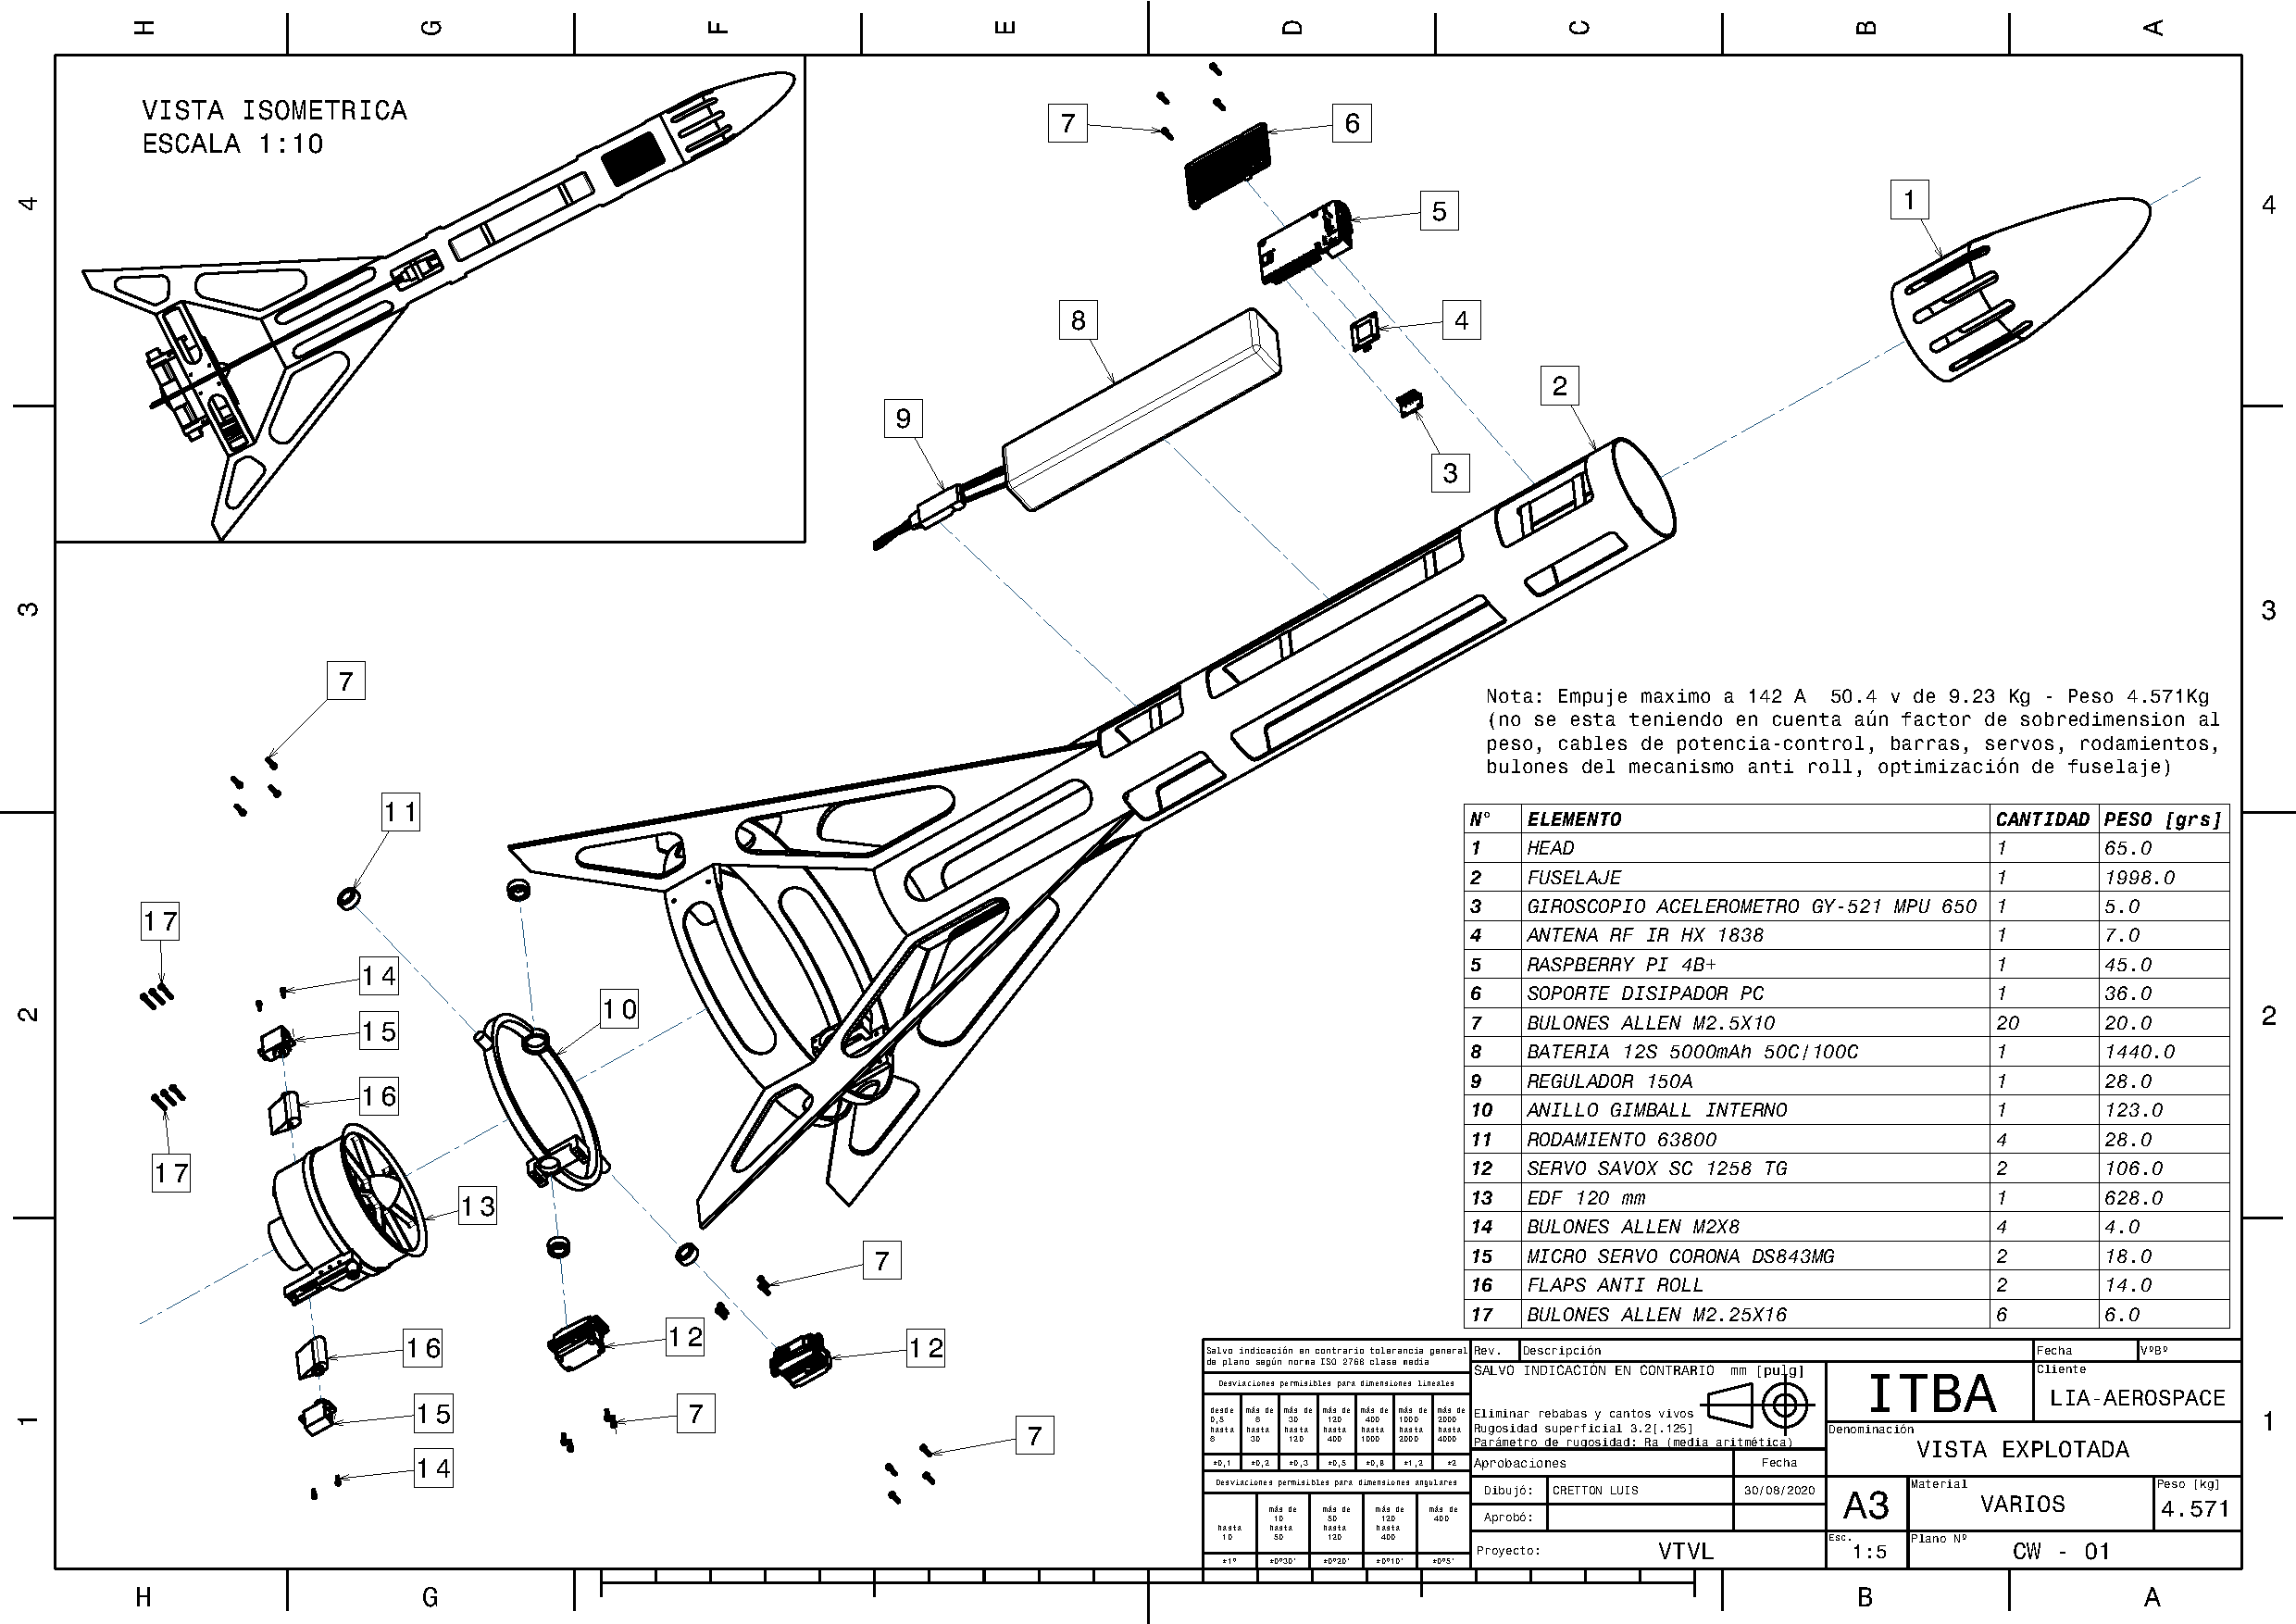
\includepdf[angle=90]{pdf/cad/Vista explotada 5}

\subsection{Diseño final - Imágenes}
% \todo{Si podemos quitar imagenes mejor. Yo personalmente no agregaría mas imagenes a no ser que agreguen valor. No agregaria las dos imagenes del anexo solo asi todo queda junto. }
\begin{figure}[htb]
    \centering
    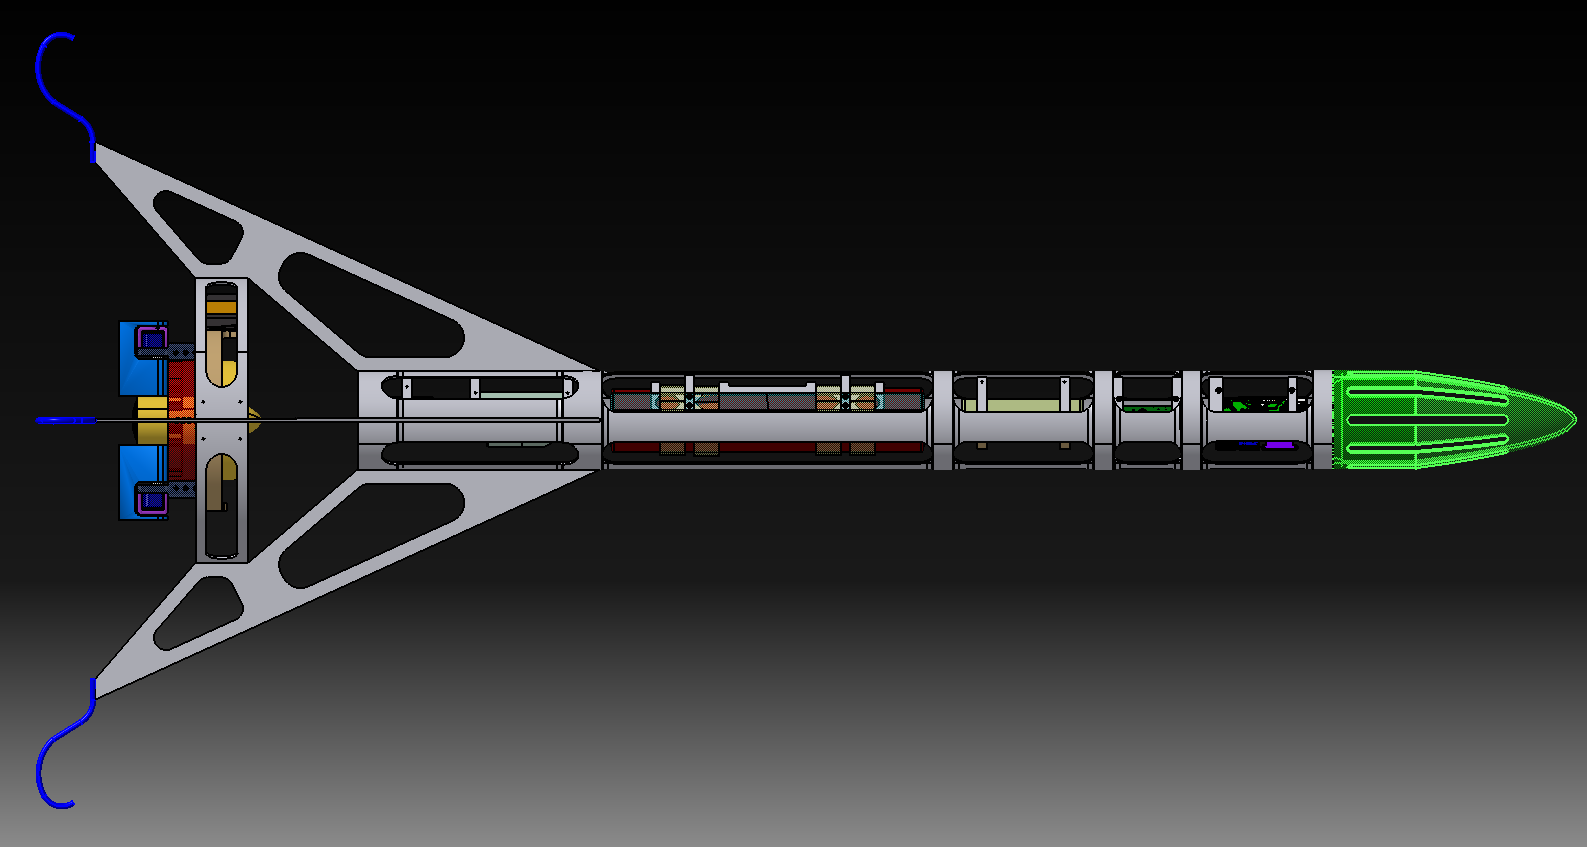
\includegraphics[width=\linewidth]{fig/design/v6}
    \caption{Prototipo final, vista de frente, batería principal en el núcleo, incorporación de batería secundaria, aviónica en la parte superior, nariz aerodinámica, sistema anti-rolido en la parte inferior por derivación del flujo, patas y fuselaje vaciado, sistema de suspensión elástico.}
    \label{fig:design/v6}
\end{figure}

\begin{figure}[htb]
    \centering
    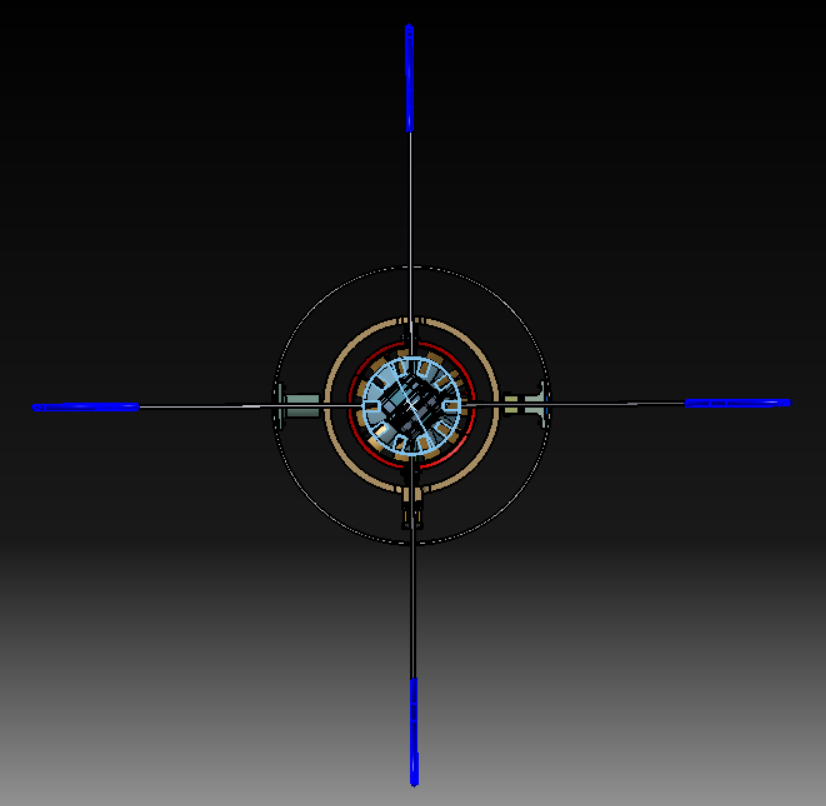
\includegraphics[width=0.8\linewidth]{fig/design/v6_1}
    \caption{Prototipo final, vista superior.}
    \label{fig:design/v6_1}
\end{figure}


\begin{figure}[htb]
    \centering
    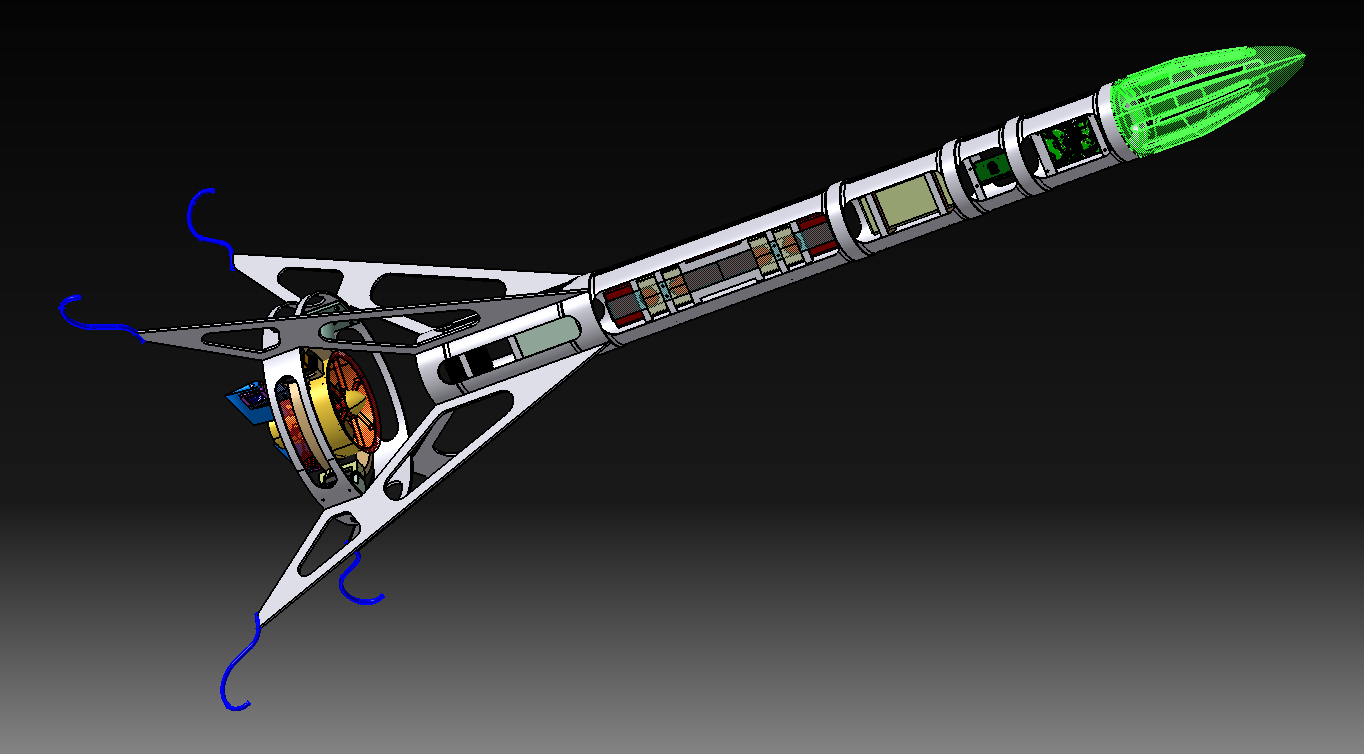
\includegraphics[width=0.8\linewidth]{fig/design/v6_2}
    \caption{Prototipo final vista isométrica axonométrica.}
    \label{fig:design/v6_2}
\end{figure}



\begin{figure}[htb]
    \centering
    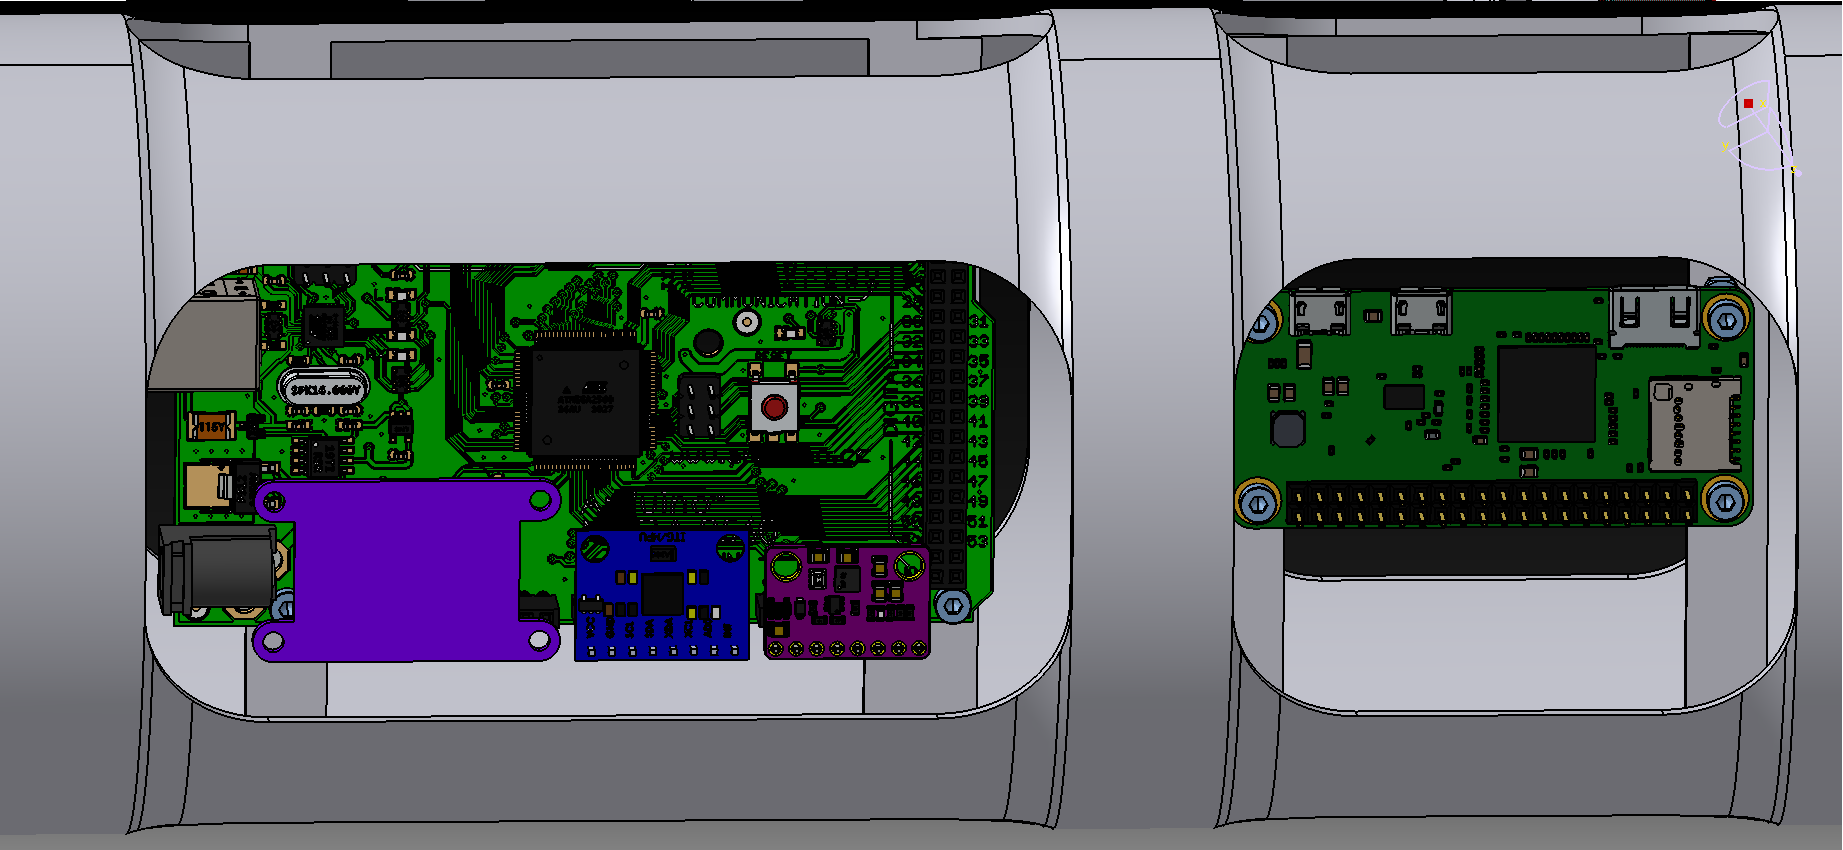
\includegraphics[width=0.8\linewidth]{fig/design/v6_4}
    \caption{Prototipo final, detalle aviónica.}
    \label{fig:design/v6_4}
\end{figure}


\begin{figure}[htb]
    \centering
    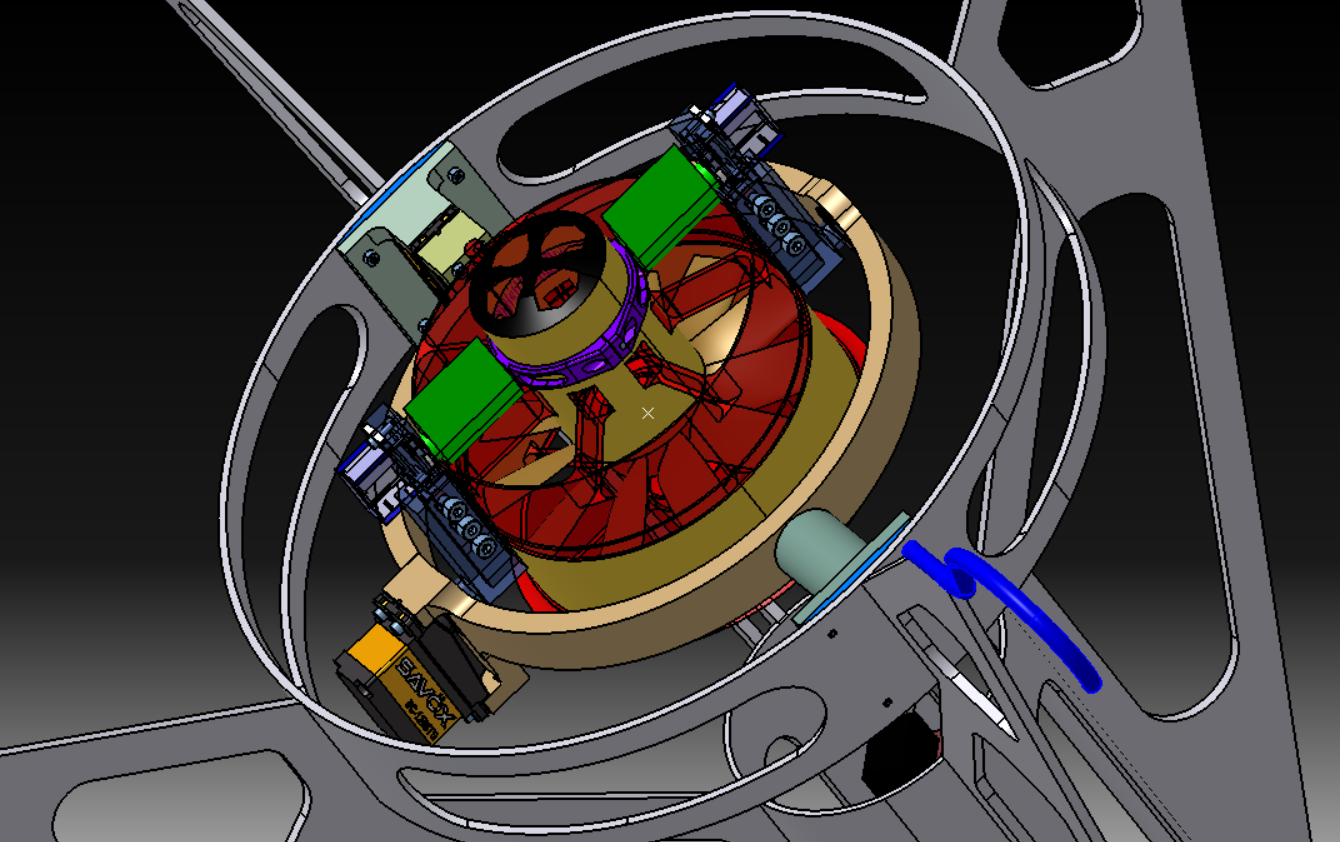
\includegraphics[width=0.8\linewidth]{fig/design/v6_6}
    \caption{Prototipo final detalle de componentes.}
    \label{fig:design/v6_6}
\end{figure}

\null\newpage
\clearpage

\subsection{Ensamblaje final - Fotos}

\begin{figure}[htb]
    \centering
    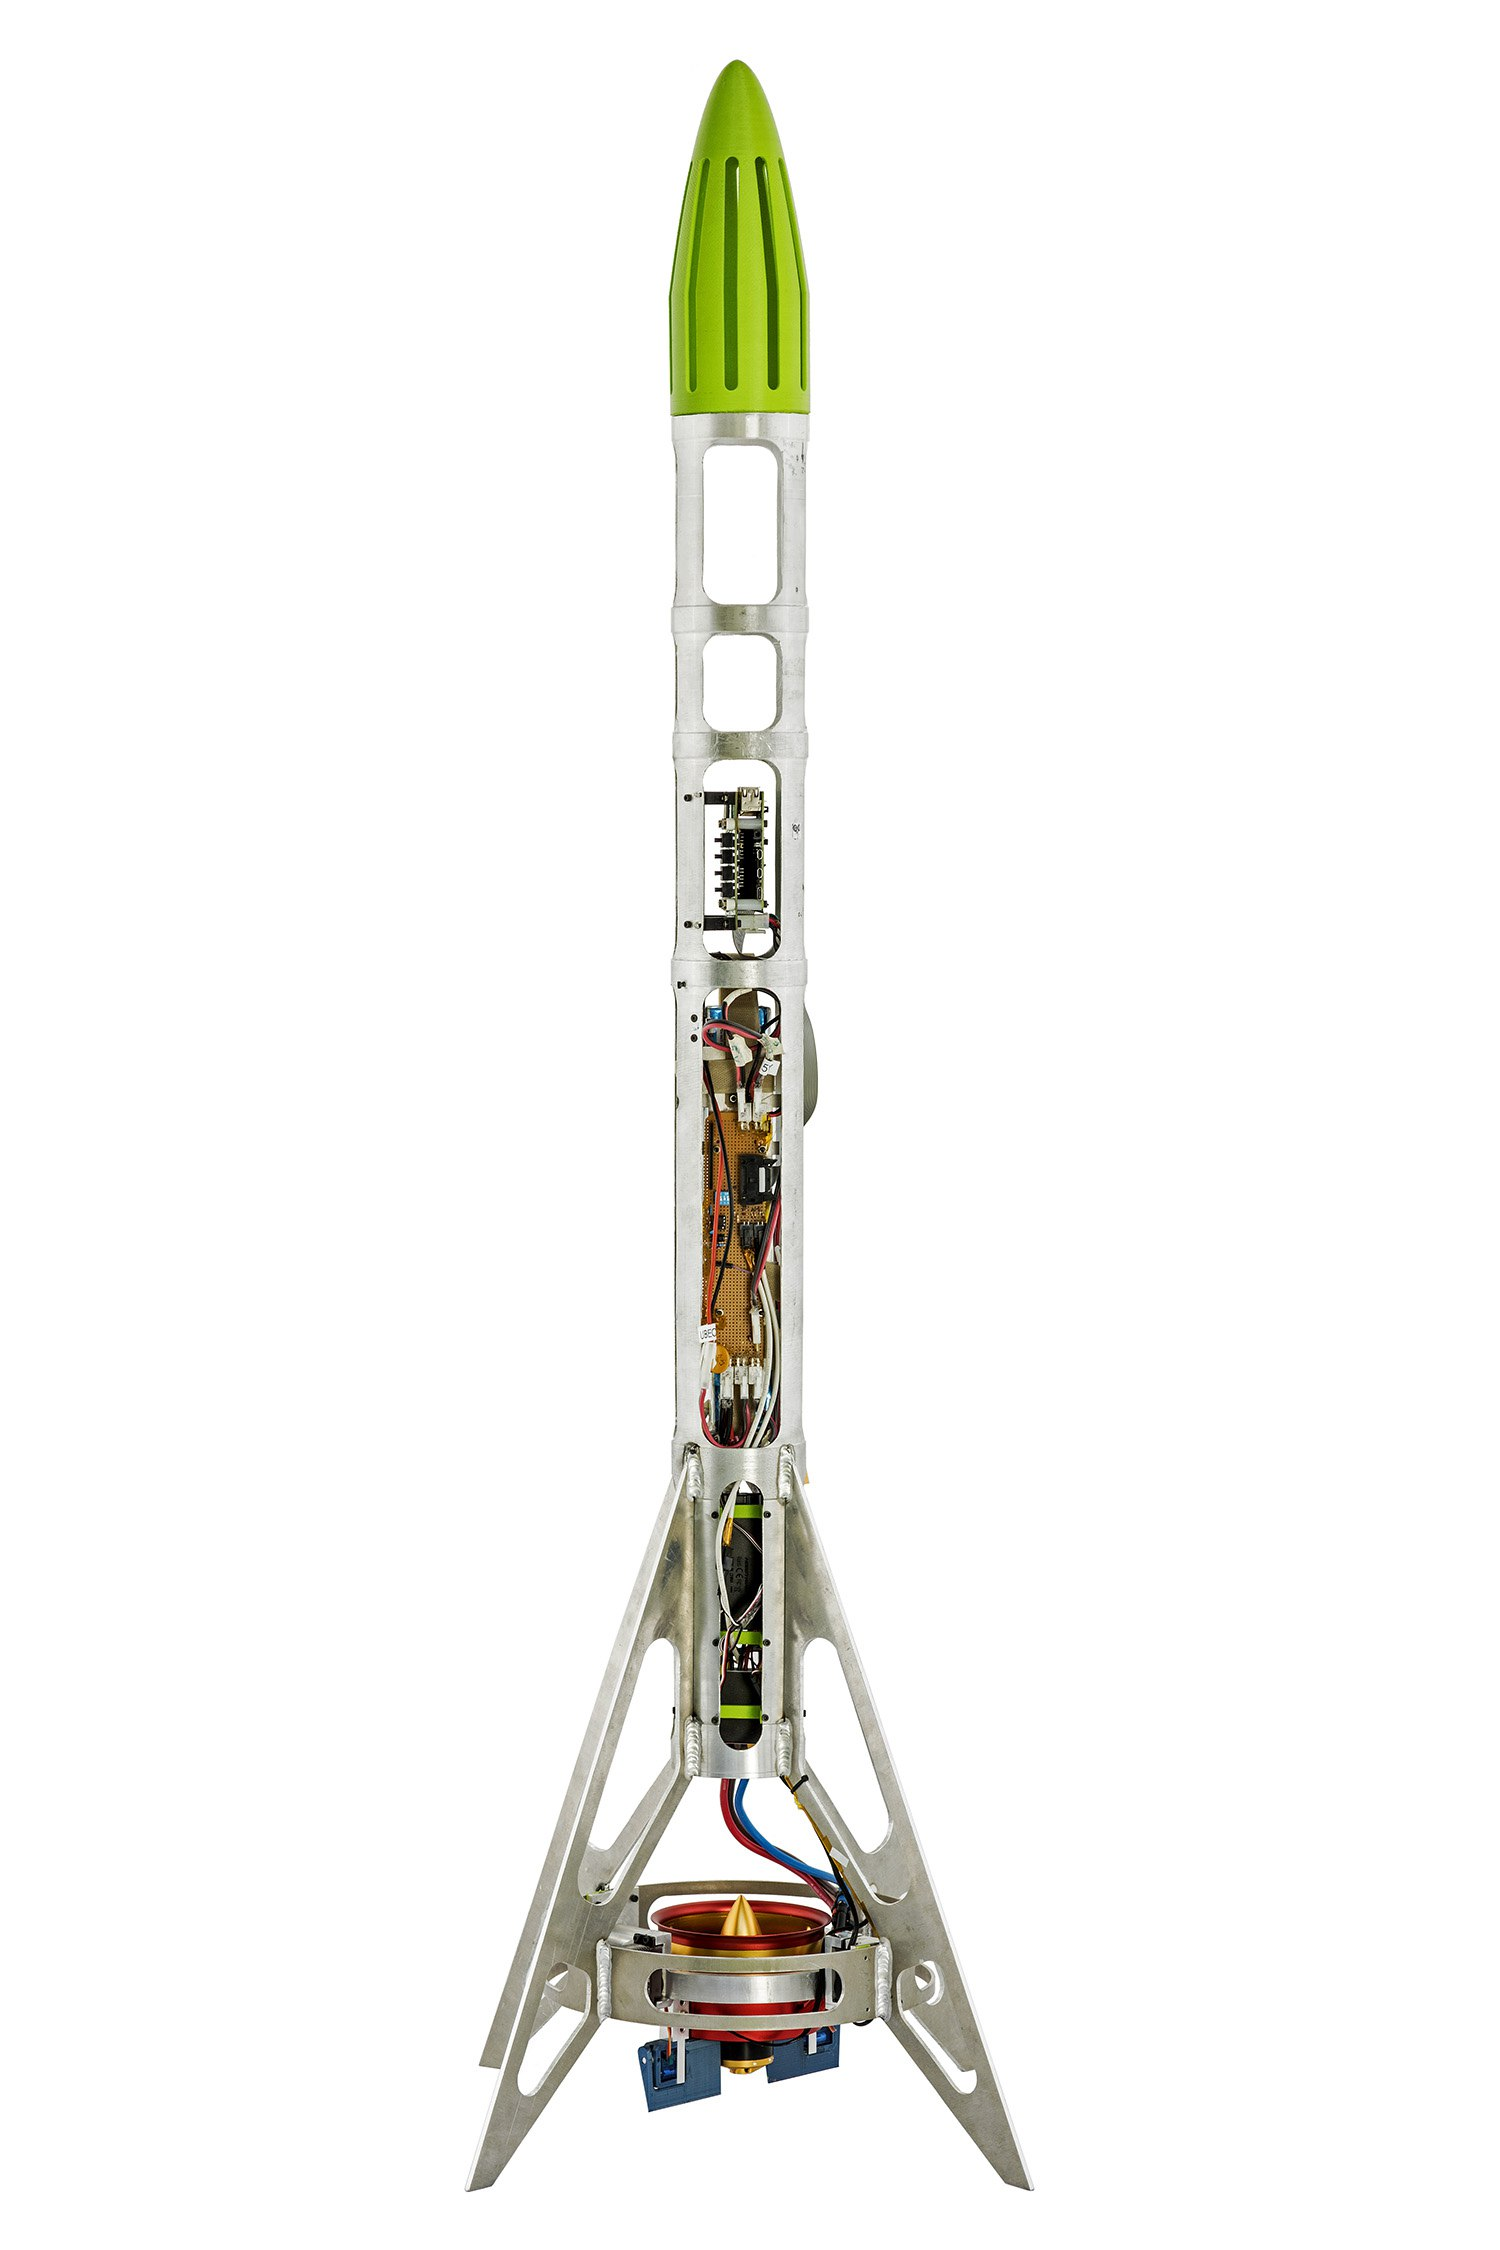
\includegraphics[width=\linewidth]{fig/hq/wide_plane_bonete.jpg}
    \caption{PFoto del conjunto armado.}
    \label{fig:hq/wide_plane_bonete}
\end{figure}

\begin{figure}[htb]
    \centering
    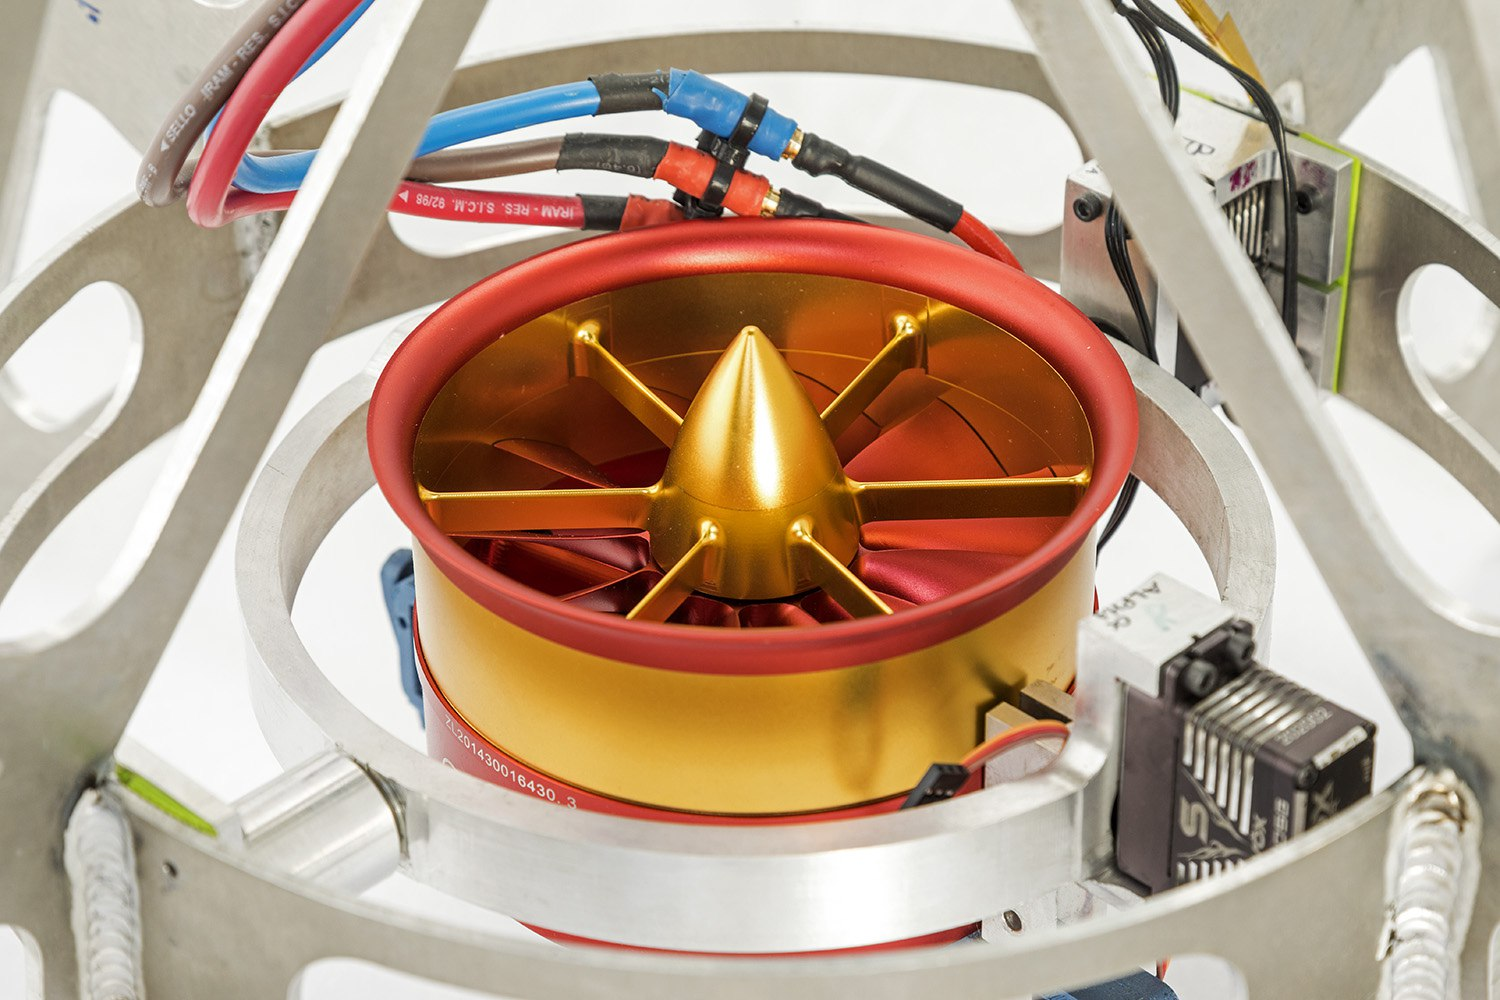
\includegraphics[width=\linewidth]{fig/hq/gimbal_close.jpg}
    \caption{Conjunto cardán, servos y soportes de gimbal externo.}
    \label{fig:hq/gimbal_close}
\end{figure}

\begin{figure}[htb]
    \centering
    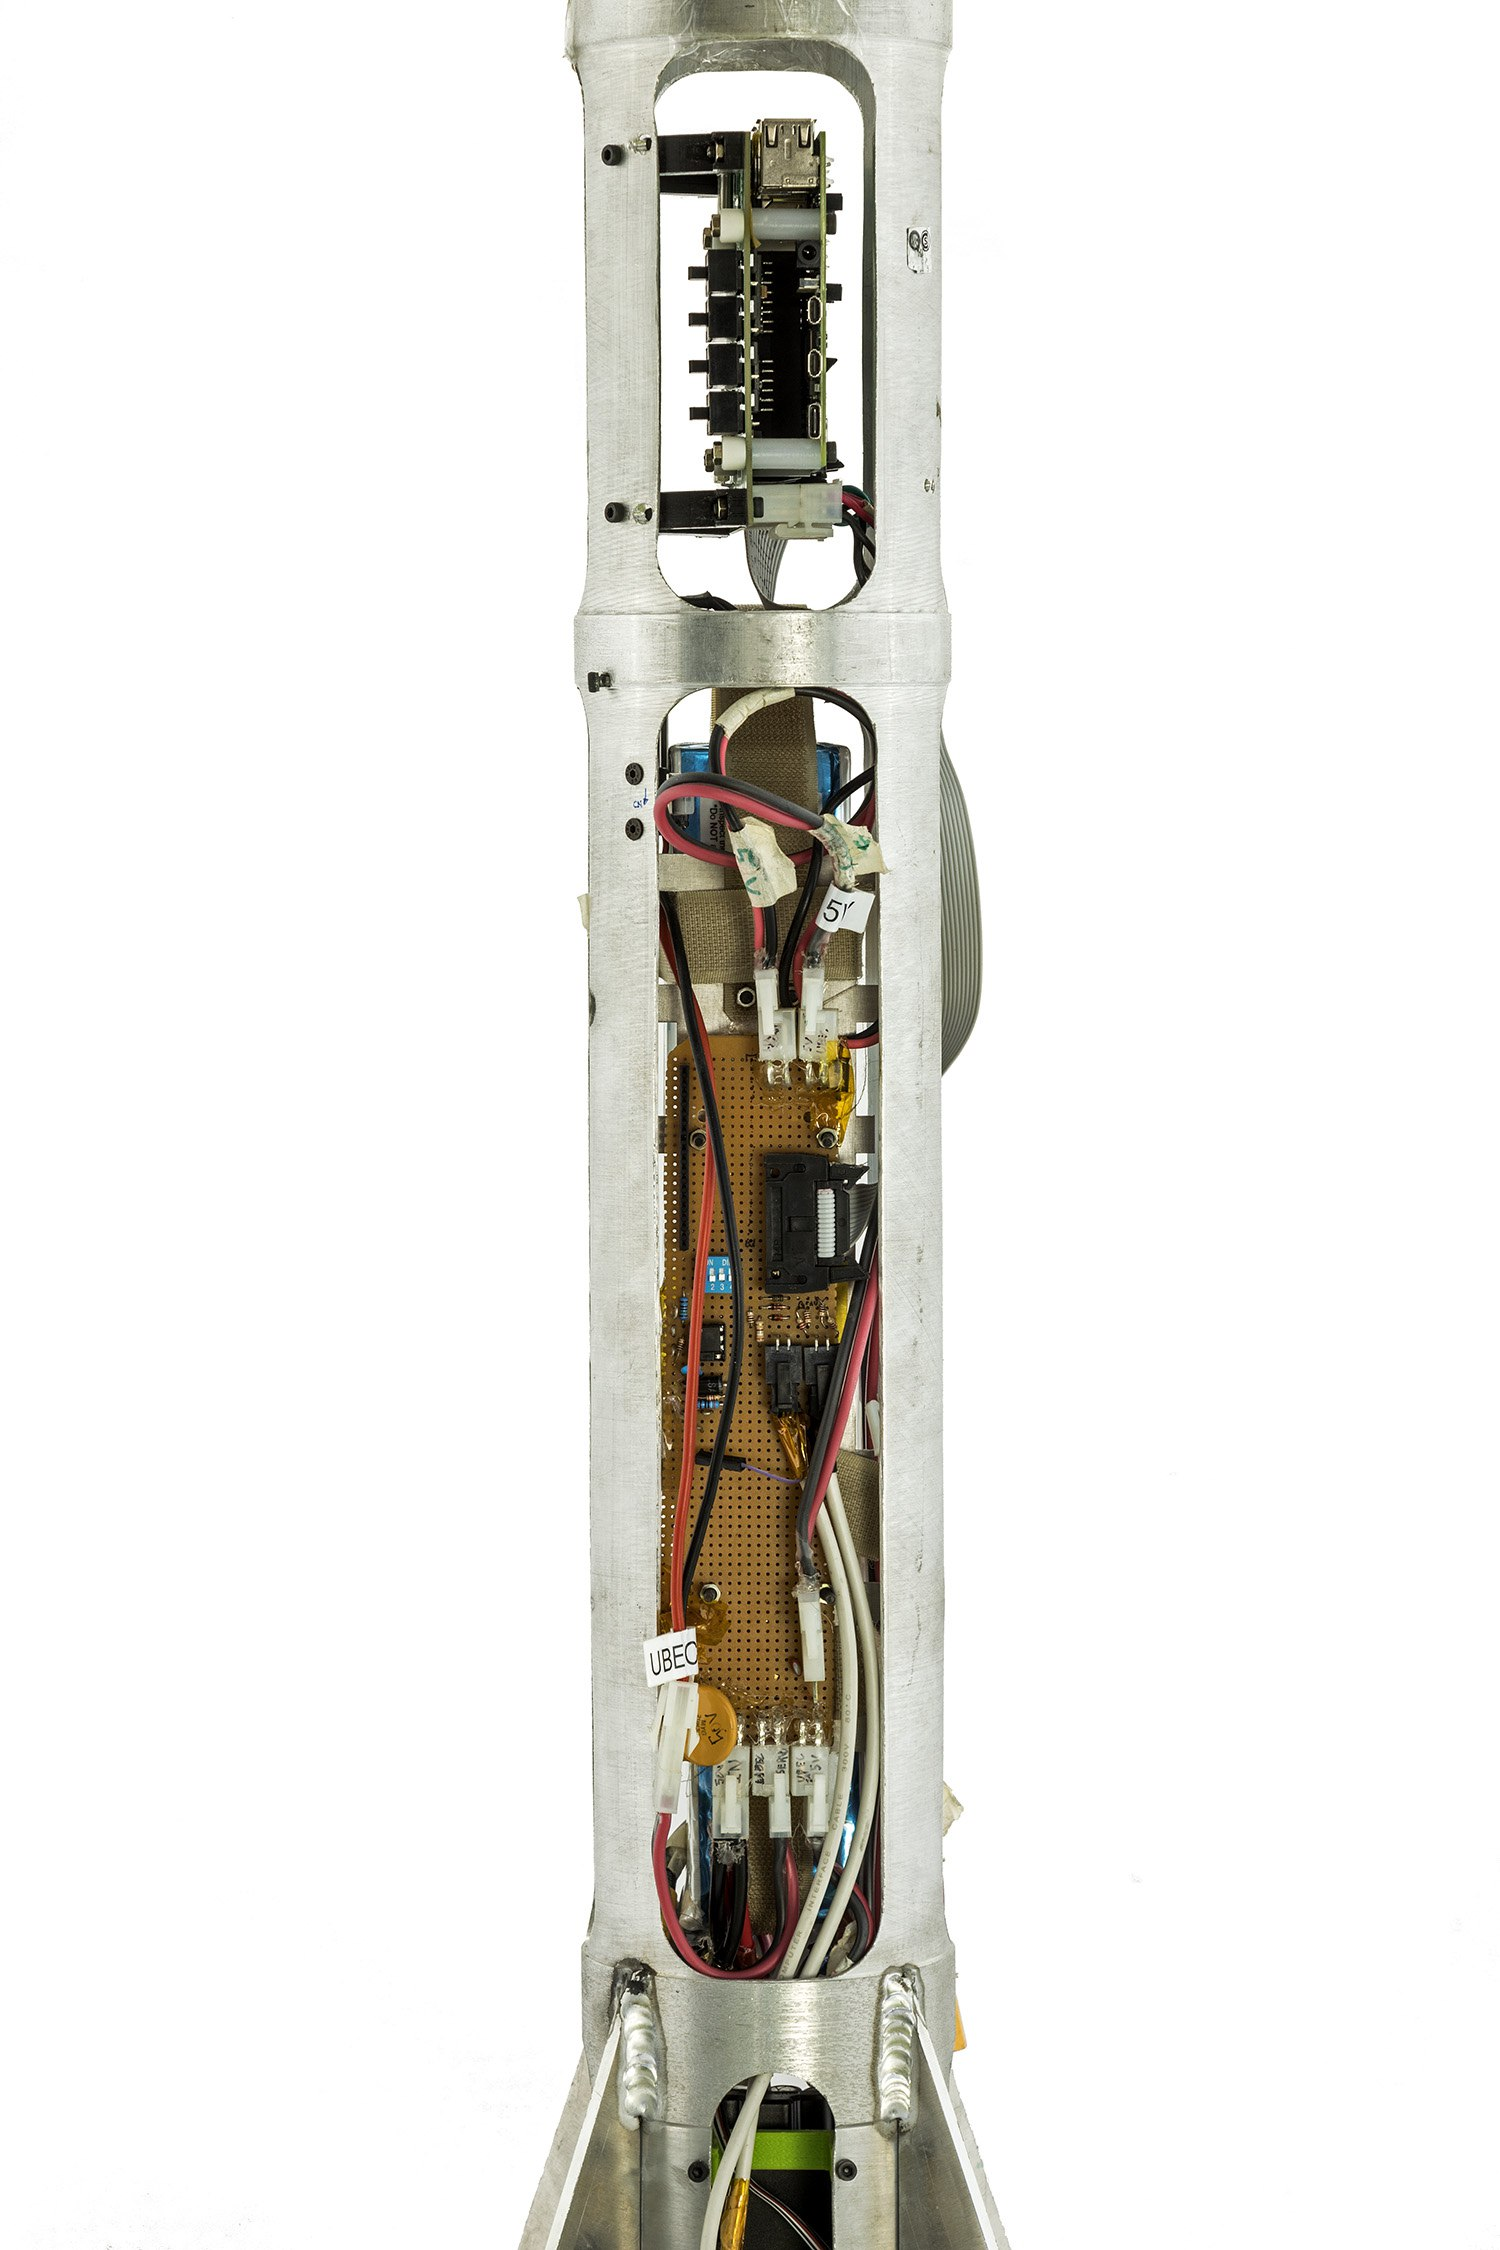
\includegraphics[width=\linewidth]{fig/hq/electronics.jpg}
    \caption{Conjuntos electrónica y cableado.}
    \label{fig:hq/electronics}
\end{figure}

\begin{figure}[htb]
    \centering
    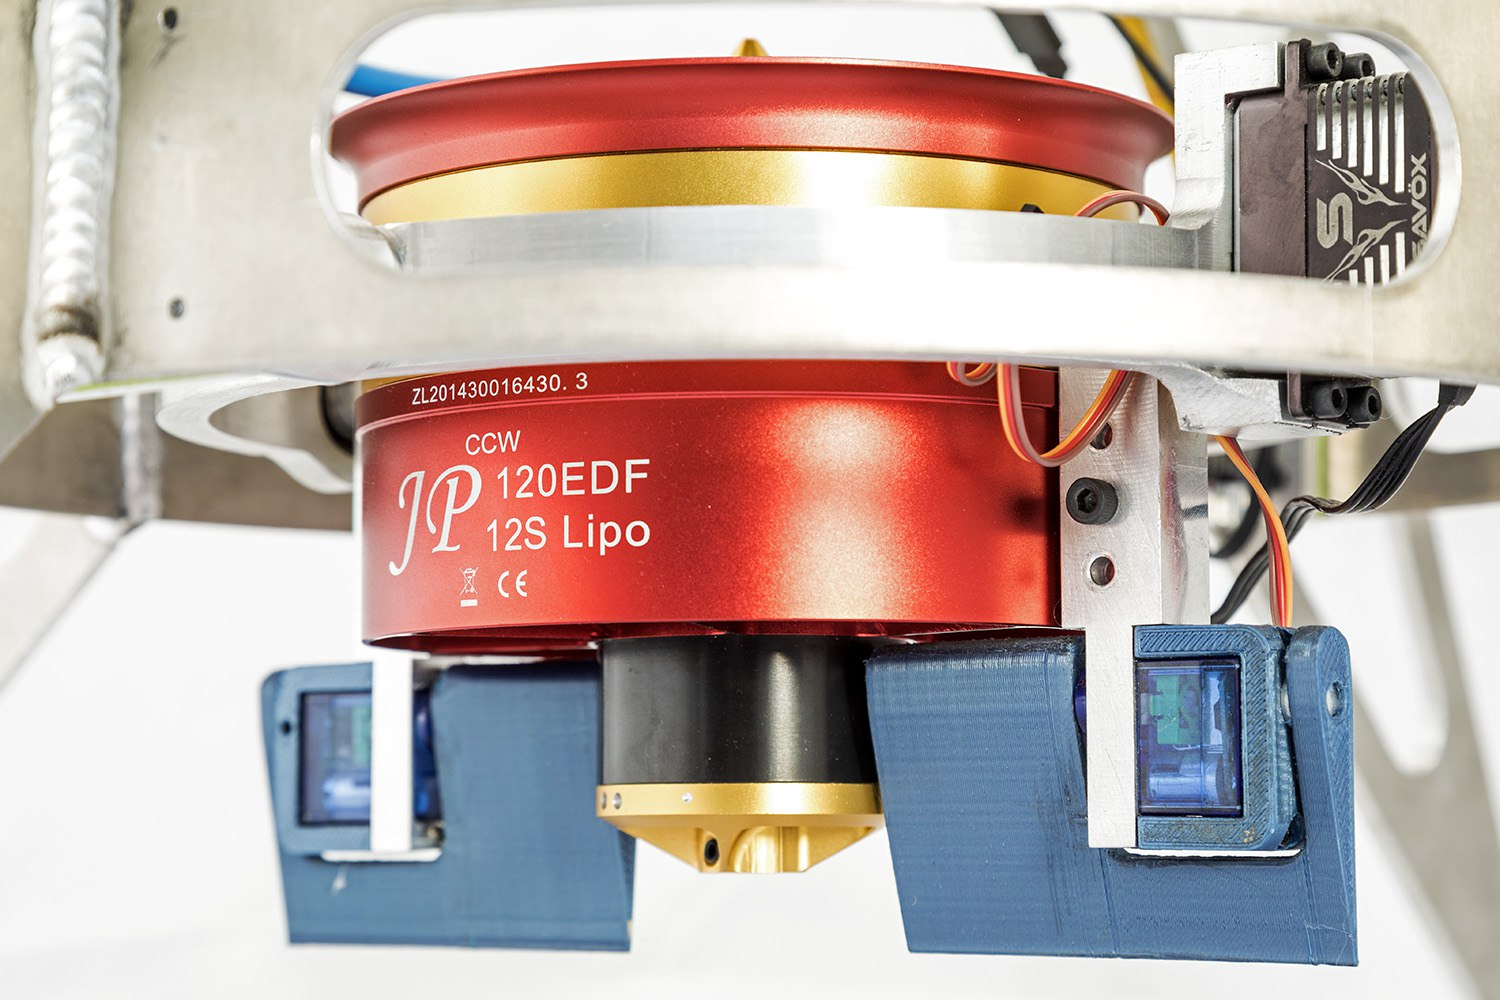
\includegraphics[width=\linewidth]{fig/hq/flaps.jpg}
    \caption{Vista inferior del conjunto cardán y flaps.}
    \label{fig:hq/flaps}
\end{figure}

\begin{figure}[htb]
    \centering
    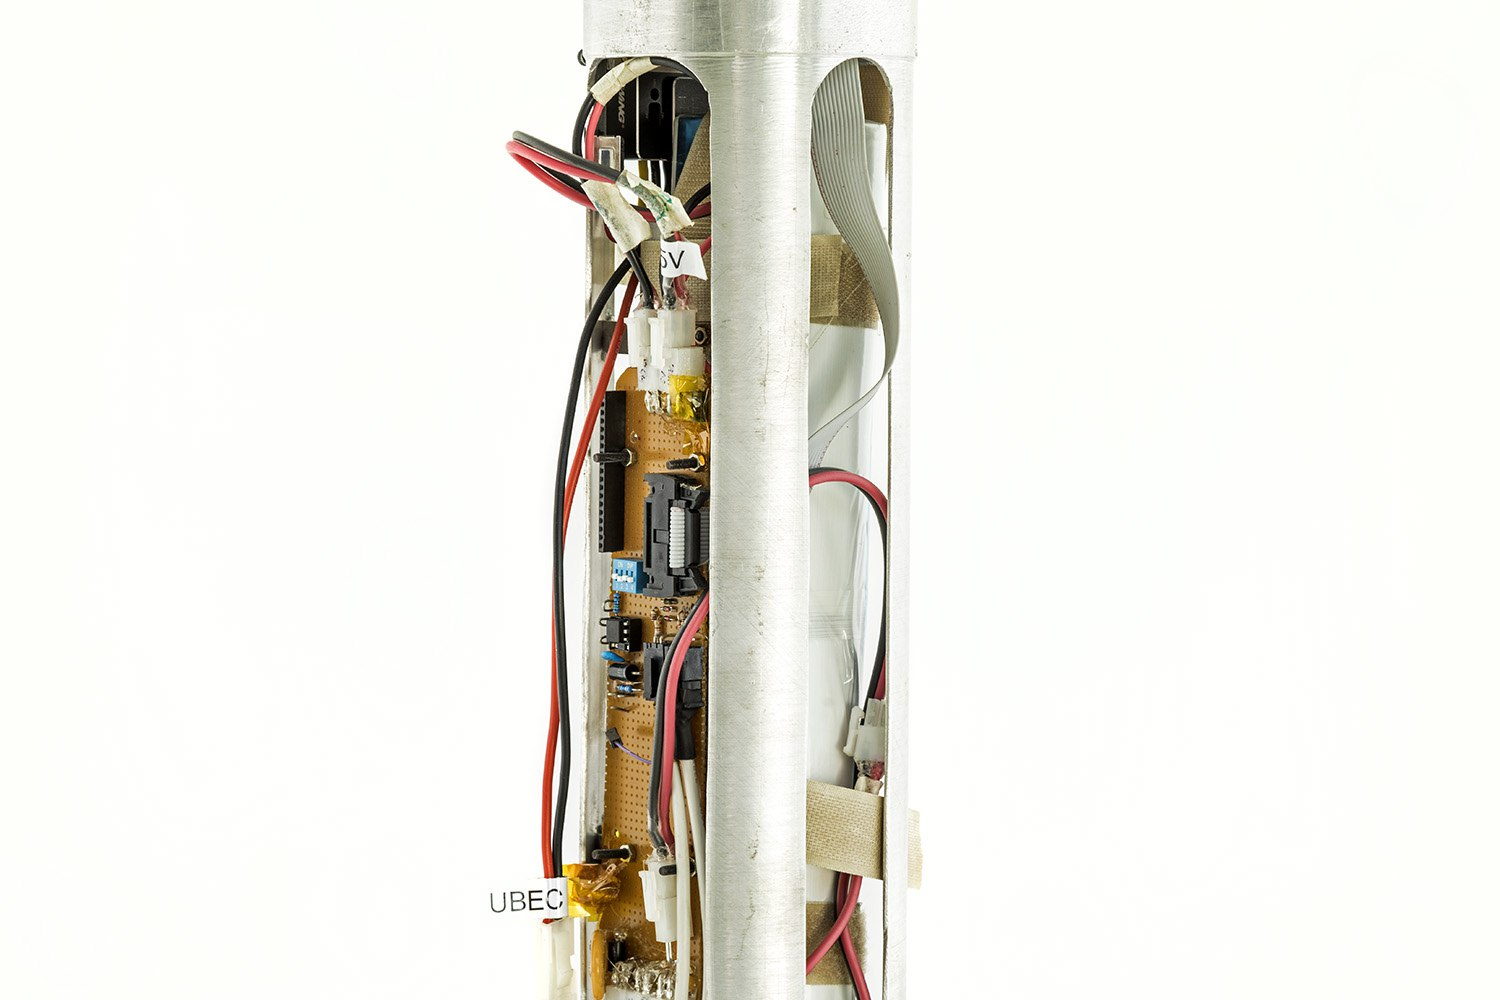
\includegraphics[width=\linewidth]{fig/hq/backpcb.jpg}
    \caption{Plano detalle de la placa electrónica de potencia.}
    \label{fig:hq/backpcb}
\end{figure}
